\chapter{Methodology}

The main algorithm is comprised of two primary steps: data preprocessing and the behavior algorithm. In the data preprocessing phase, regions are converted into points by computing the centroids of their overlaps. The behavior algorithm phase utilizes these computed points to generate the complete path.

\section{Data Preprocessing}


Data preprocessing is a pivotal step in the research methodology, especially in the context of coverage path planning for weed removal in agricultural fields. This section delineates the comprehensive preprocessing procedures employed to ensure the precision and efficacy of the data used in the subsequent analysis.

\vspace{3mm}  


\textbf{Data Acquisition: }
The initial phase of preprocessing involves the acquisition of data pertaining to the weed positions within the field. This data collection is facilitated through the use of a drone for pinpointing the locations of weeds. The drone performs a systematic survey of the field, capturing high-resolution images to detect weed positions. The resultant data is then utilized as input for the coverage path planning module. Due to the developmental status of the drone, the current implementation involves manual data acquisition using a real-time kinematic GPS (RTK) system. The RTK system offers centimeter-level accuracy in pinpointing weed locations, which, for the purpose of this research, is considered sufficiently precise. 

\vspace{3mm}  


\textbf{Handling Data Uncertainty: }
In a practical scenario, the drone's output would include positional data of weeds along with an associated uncertainty measure, reflecting the inherent imprecision of the system. However, given the reliance on RTK data for this research phase, we assume perfect positional accuracy. This uncertainty measure will be used to define the regions of influence for each weed, ensuring that the coverage path planning algorithm accounts for the imprecision in the data. 


\vspace{3mm}  


\textbf{Region Definition and Overlap Management: } When data points from the drone indicate weed positions, these points often come with overlapping regions due to the growth patterns of weeds like Rumex, which tend to cluster.

\vspace{3mm}  


Overlap Reduction: To address overlaps, the preprocessing algorithm calculates the centroids of overlapping regions. Points within overlapping regions are consolidated to avoid duplication, ensuring that each weed cluster is represented by a single centroid. This consolidation reduces redundancy and enhances the efficiency of the coverage path planning.

\vspace{3mm}  


Non-Overlapping Weeds: For weeds whose regions do not overlap with others, the center of each weed is directly considered as a centroid. This step ensures that isolated weeds are accurately accounted for in the data set. The centroids of both overlapping and non-overlapping regions can be visualized in the \autoref{fig:overlape}. The green points represent the weeds, green circles represent the region of the weeds, and the red points represent the centroids of the regions. 

% selected field region.
\begin{figure}
    \centering
    \begin{tabular}{cc} 
        \begin{subfigure}{0.5\textwidth}
            \centering
            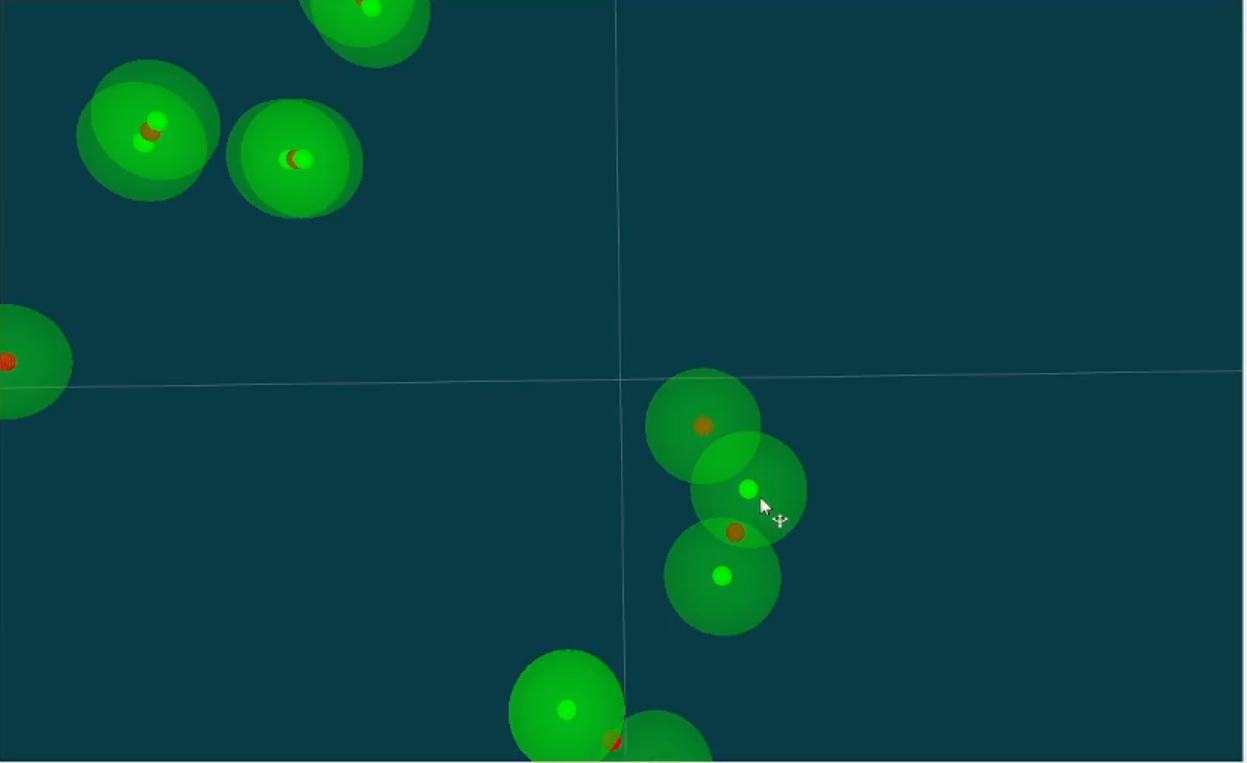
\includegraphics[width=\textwidth]{Images/Algorithm_no_obs/Centroid_1.png}
            % \caption{Selected Field Region}
        \end{subfigure} 
        &
        \begin{subfigure}{0.5\textwidth}
            \centering
            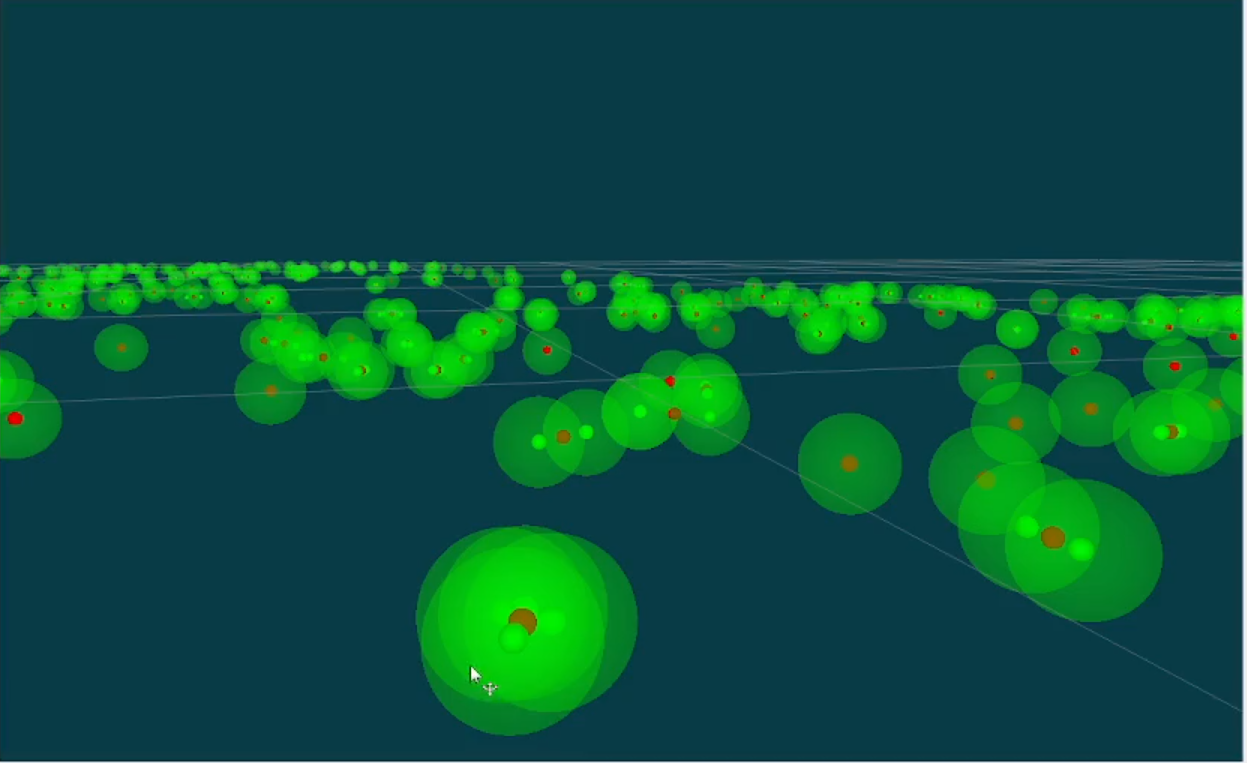
\includegraphics[width=\textwidth]{Images/Algorithm_no_obs/Centroid_2.png}
            % \caption{Points in the Region (Green)}
        \end{subfigure}
    \end{tabular}
    \caption{Centroids of overlapped regions.\label{fig:overlape}} 
\end{figure}

\vspace{3mm}  


\textbf{Data Integration and Optimization: }
By processing the data to identify centroids and manage overlaps, we achieve a significant reduction in the total number of points. Preliminary results indicate a reduction of at least 40\% in the number of data points, optimizing the dataset for coverage path planning. This reduction not only minimizes the total traversal length required for weed removal but also conserves energy and reduces redundant revisits.

\vspace{3mm}  


The processed data is then fed into the coverage path planning module, which utilizes the optimized set of points to devise an efficient path for weed removal, ensuring comprehensive coverage with minimal resource expenditure. The following figure illustrates the data preprocessing workflow, highlighting the steps taken to transform raw positional data into an optimized dataset ready for coverage path planning.

\vspace{3mm}  



This preprocessing approach ensures that the data fed into the coverage path planning algorithm is both accurate and efficient, laying a robust foundation for effective weed removal operations in agricultural fields.

